% In this section, the layer is described in some detail in terms of its specific subsystems. Describe each of the layers and its subsystems in a separate chapter/major subsection of this document. The content of each subsystem description should be similar. Include in this section any special considerations and/or trade-offs considered for the approach you have chosen.

%%%%%%%%%%%%%%%%%%%%%%%%%%%%%%%%%%%%%%%%%%%%%%%%%%%%%%%%%%%%%%%%%%%%%%%%%%%%

\subsection{Speed Control}
% This section should be a general description of a particular subsystem for the given layer. For most subsystems, an extract of the architectural block diagram with data flows is useful. This should consist of the subsystem being described and those subsystems with which it communicates.
The speed control subsystem manages the power of each motor to maintain a specific set speed. It receives feedback from the odometer and crash prevention to ensure safe operation.

%   Change the graphic here. Put your image in the 'images' folder
%   and update the name from 'images/test_image' to your image name
\begin{figure}[h!]
	\centering
 	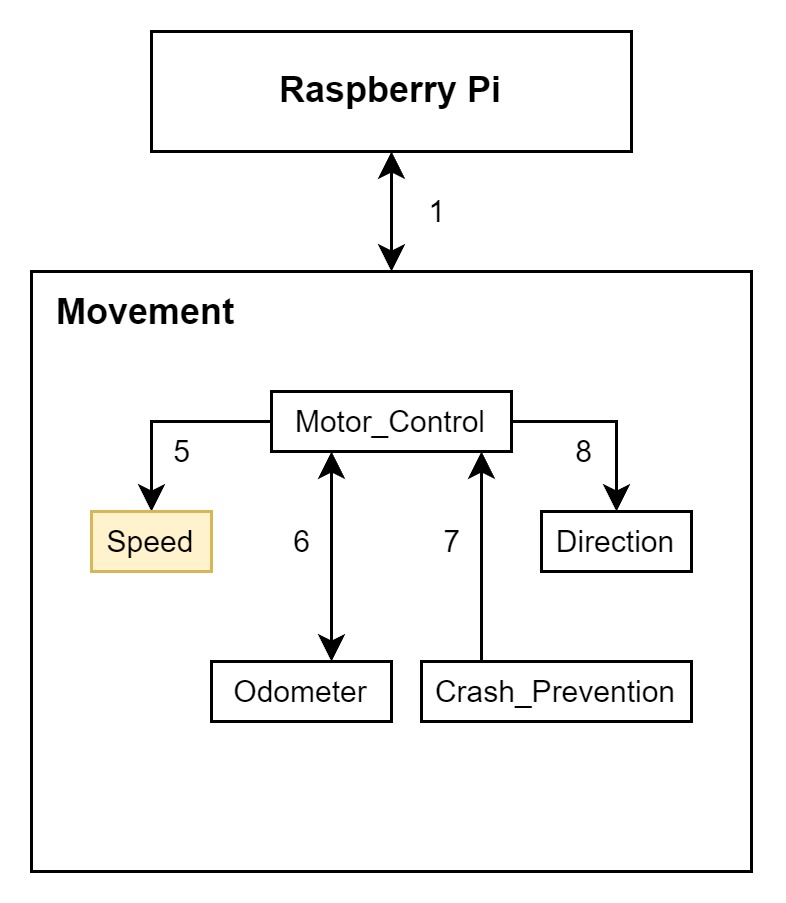
\includegraphics[width=0.45\textwidth]{images/movement/speed.jpg}
 \caption{Movement Subsystem - Speed Control} % Be sure to change the caption
\end{figure}

\subsubsection{Assumptions}
% Any assumptions made in the definition of the subsystem should be listed and described. Pay particular attention to assumptions concerning interfaces and interactions with other layers.
The motor driver supports PWM input to control motor speed. The odometer feedback is accurate within 10\% from wheel encoder measurements \cite{Zhang2020}. Communication latency between the TM4C and Raspberry Pi isn't noticeable for real-time feedback.

\subsubsection{Responsibilities}
% Each of the responsibilities/features/functions/services of the subsystem as identified in the architectural summary must be expanded to more detailed responsibilities. These responsibilities form the basis for the identification of the finer-grained responsibilities of the layer's internal subsystems. Clearly describe what each subsystem does.
Adjust motor PWM signals to match the target speed set. Monitor odometer feedback to ensure the actual speed matches the desired speed. Stop the speed if a collision is detected.

\subsubsection{Subsystem Interfaces}
% Each of the inputs and outputs for the subsystem are defined here. Create a table with an entry for each labeled interface that connects to this subsystem. For each entry, describe any incoming and outgoing data elements will pass through this interface.

\begin {table}[H]
\caption {Movement Subsystem - Speed Control} 
\begin{center}
    \begin{tabular}{ | p{1cm} | p{6cm} | p{3cm} | p{3cm} |}
    \hline
    ID & Description & Inputs & Outputs \\ \hline
    \#5 & Pulse Width Modulation (PWM) & Power In & N/A \\ \hline
    \end{tabular}
\end{center}
\end{table}

\newpage

%%%%%%%%%%%%%%%%%%%%%%%%%%%%%%%%%%%%%%%%%%%%%%%%%%%%%%%%%%%%%%%%%%%%%%%%%%%%%%%%%%

\subsection{Direction Control}
The direction control subsystem manages the robot's steering by adjusting the motor signals for the left and right wheels. It receives feedback from the steering sensors and ensures the rover follows the correct path.

\begin{figure}[h!]
	\centering
 	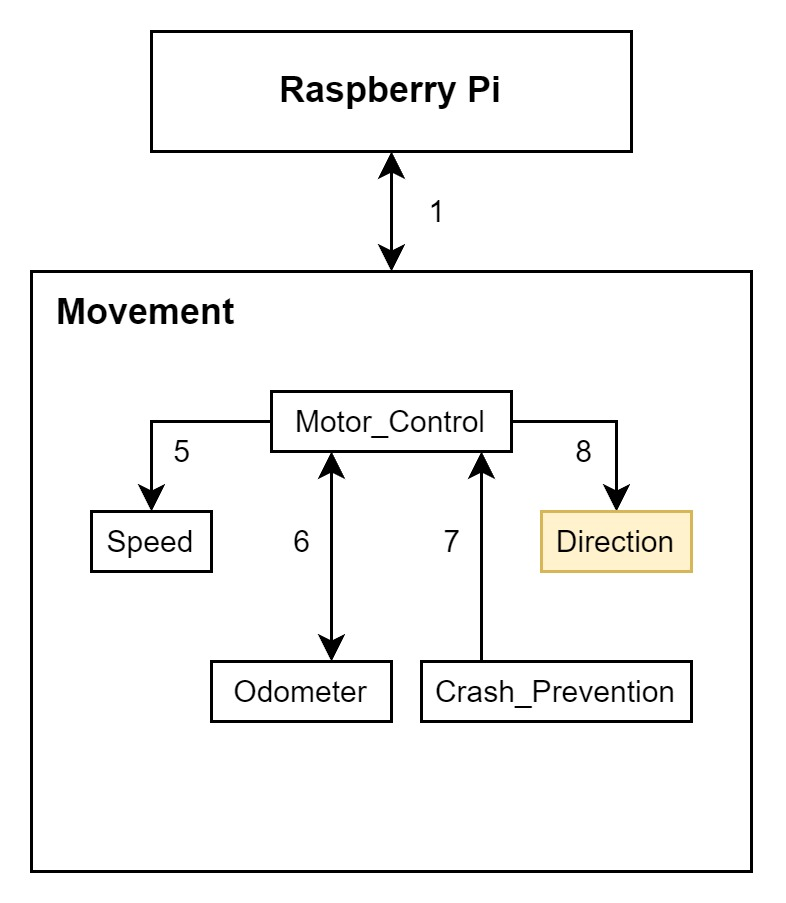
\includegraphics[width=0.45\textwidth]{images/movement/direction.jpg}
 \caption{Movement Subsystem - Direction Control} % Be sure to change the caption
\end{figure}

\subsubsection{Assumptions}
The motor driver supports PWM input to control motor direction. The steering feedback system is accurate within 5\% from LIDAR measurements \cite{Epton2012}. Communication latency between the TM4C and Raspberry Pi is minimal for real-time control.

\subsubsection{Responsibilities}
Adjust motor PWM signals to steer the robot in the desired direction. Monitor steering feedback to ensure the robot is following the intended path. Correct any misalignment detected by the steering sensors.

\subsubsection{Subsystem Interfaces}

\begin {table}[H]
\caption {Movement Subsystem - Direction Control} 
\begin{center}
    \begin{tabular}{ | p{1cm} | p{6cm} | p{3cm} | p{3cm} |}
    \hline
    ID & Description & Inputs & Outputs \\ \hline
    \#8 & Pulse Width Modulation (PWM) & Power In & N/A \\ \hline
    \end{tabular}
\end{center}
\end{table}

\newpage

%%%%%%%%%%%%%%%%%%%%%%%%%%%%%%%%%%%%%%%%%%%%%%%%%%%%%%%%%%%%%%%%%%%%%%%%%%%%%%%%%%

\subsection{Motor Control}
The motor control subsystem manages the power supplied to the motors to achieve the desired movement. It receives feedback from the motor encoders and adjusts the motor signals to control both speed and direction.

\begin{figure}[h!]
	\centering
 	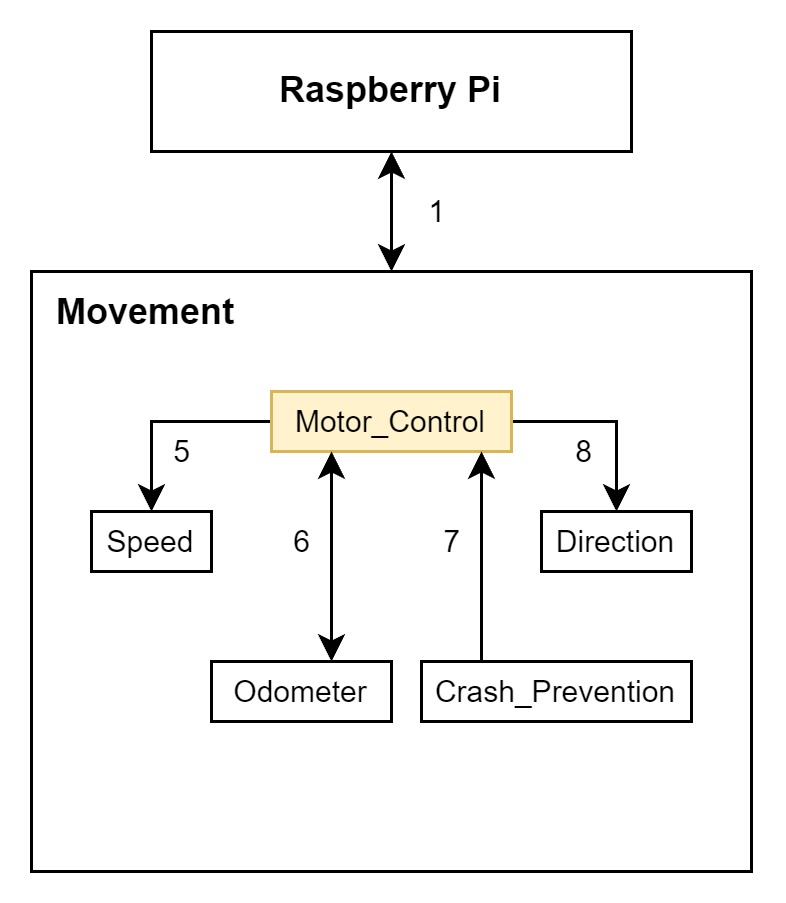
\includegraphics[width=0.45\textwidth]{images/movement/motor_control.jpg}
 \caption{Movement Subsystem - Motor Control} % Be sure to change the caption
\end{figure}

\subsubsection{Assumptions}
The motor driver supports both PWM and direction control signals to drive motor speed and direction \cite{DimensionEngineeringSabertooth2x25}. The motor encoders provide accurate feedback to control speed and direction adjustments. Communication latency between the TM4C and Raspberry Pi does not impact real-time motor control.

\subsubsection{Responsibilities}
Control motor power to achieve the desired speed and direction. Monitor motor feedback to ensure correct operation and make adjustments when necessary. Handle error states, such as motor stall or failure, and stop the motors if a critical fault is detected.

\subsubsection{Subsystem Interfaces}

\begin{table}[H]
\caption{Movement Subsystem - Motor Control} 
\begin{center}
    \begin{tabular}{ | p{0.8cm} | p{6cm} | p{4cm} | p{3cm} |}
    \hline
    ID & Description & Inputs & Outputs  \\ \hline
    \#5 & Pulse Width Modulation (PWM) & N/A & Power Output \\ \hline
    \#6 & General Purpose Input Output (GPIO) & Odometer Feedback  & Odometer Control \\ \hline
    \#7 & General Purpose Input Output (GPIO) & Crash Detect & N/A \\ \hline
    \#8 & Pulse Width Modulation (PWM) & N/A & Power Output \\ \hline
    \end{tabular}
\end{center}
\end{table}

\newpage

%%%%%%%%%%%%%%%%%%%%%%%%%%%%%%%%%%%%%%%%%%%%%%%%%%%%%%%%%%%%%%%%%%%%%%%%%%%%%%%%%%

\subsection{Odometer}
The odometer subsystem is responsible for measuring the distance traveled by the vehicle. It provides feedback to the motor control subsystem to help adjust the speed and ensure accurate movement over time.

\begin{figure}[h!]
	\centering
 	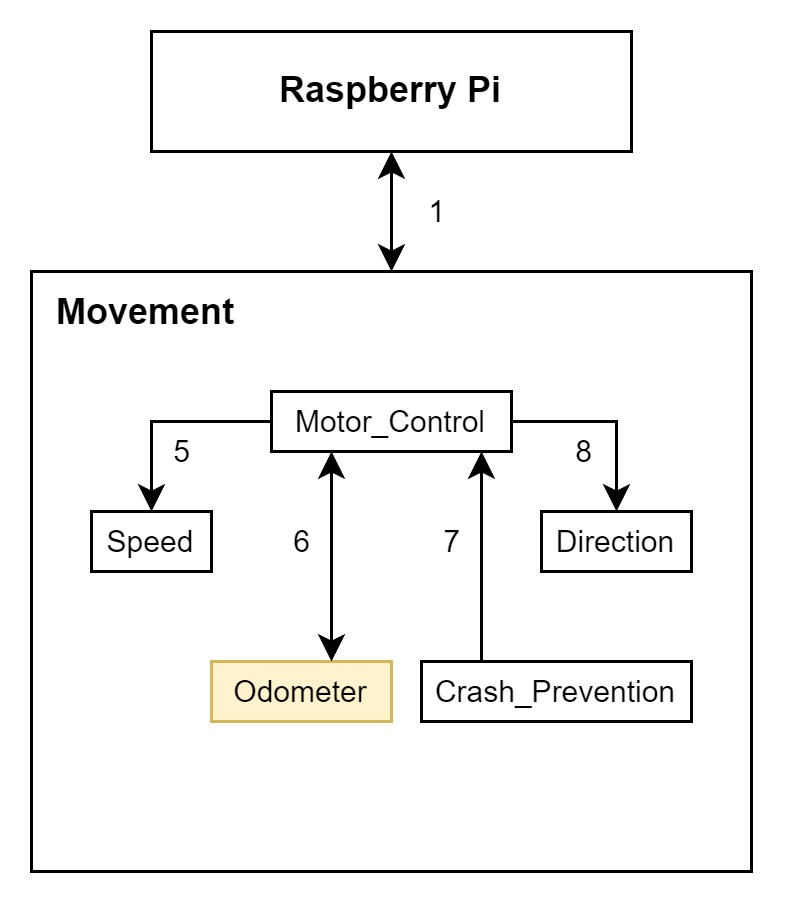
\includegraphics[width=0.45\textwidth]{images/movement/odometer.jpg}
 \caption{Movement Subsystem - Odometer} % Be sure to change the caption
\end{figure}

\subsubsection{Assumptions}
The odometer system uses wheel encoders and LIDAR to measure the distance traveled. The feedback is accurate within 10\% for distance measurement \cite{Zhang2020} \cite{Epton2012}. The odometer data is updated in real time, with no significant communication delays between the TM4C and Raspberry Pi affecting its accuracy.

\subsubsection{Responsibilities}
Measure the distance traveled by the vehicle based on wheel rotations. Provide real-time feedback to the motor control subsystem to adjust the speed accordingly. Alert the system if abnormal readings are detected, such as wheel slippage or encoder malfunction.

\subsubsection{Subsystem Interfaces}

\begin{table}[H]
\caption{Movement Subsystem - Odometer} 
\begin{center}
    \begin{tabular}{ | p{0.8cm} | p{6cm} | p{3cm} | p{4cm} |}
    \hline
    ID & Description & Inputs & Outputs  \\ \hline
    \#6 & General Purpose Input Output (GPIO) & Odometer Control & Odometer Feedback \\ \hline
    \end{tabular}
\end{center}
\end{table}

\newpage

%%%%%%%%%%%%%%%%%%%%%%%%%%%%%%%%%%%%%%%%%%%%%%%%%%%%%%%%%%%%%%%%%%%%%%%%%%%%%%%%%%

\subsection{Crash Detection}
The crash detection subsystem is responsible for identifying any potential collisions or obstacles in the vehicle's path. It monitors sensor data to detect obstacles or sudden changes in velocity that may indicate a crash or near-crash event.

\begin{figure}[h!]
	\centering
 	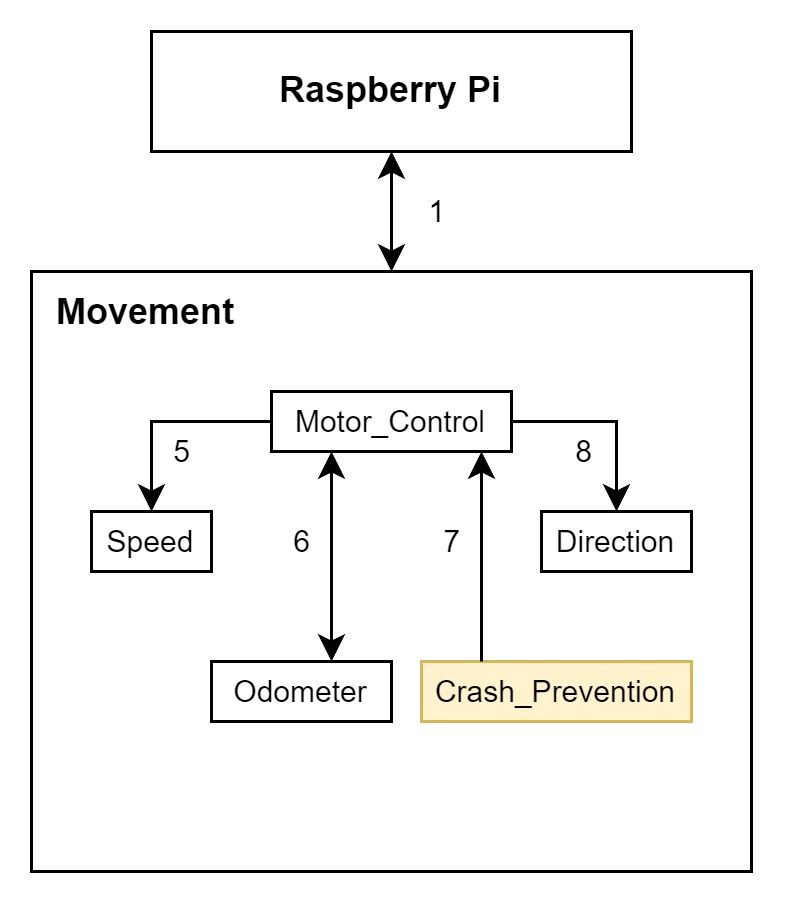
\includegraphics[width=0.45\textwidth]{images/movement/crash_prevention.jpg}
 \caption{Movement Subsystem - Crash Detection} % Be sure to change the caption
\end{figure}

\subsubsection{Assumptions}
The crash detection system uses a combination of proximity sensors and accelerometers to detect obstacles and sudden impacts \cite{Hassan2012}.The sensor system is accurate within a range of 5 cm for obstacle detection, and the accelerometers can detect changes in velocity. Communication latency between the TM4C and Raspberry Pi is minimal and does not affect real-time collision detection.

\subsubsection{Responsibilities}
Monitor sensor data to detect any obstacles or sudden changes in velocity. Alert the motor control subsystem to stop or adjust the vehicle's movement if a crash is detected. Ensure that the vehicle responds promptly to prevent further damage or injury in case of a collision.

\subsubsection{Subsystem Interfaces}

\begin {table}[H]
\caption {Movement Subsystem - Crash Detection} 
\begin{center}
    \begin{tabular}{ | p{1cm} | p{6cm} | p{3cm} | p{3cm} |}
    \hline
    ID & Description & Inputs & Outputs \\ \hline
    \#7 & General Purpose Input Output (GPIO) & Crash Detect & N/A \\ \hline
    \end{tabular}
\end{center}
\end{table}

\newpage
